\documentclass[a4paper, 10pt, twocolumn]{article}
\usepackage[a4paper, left=.7in, right=.7in, top=1in]{geometry} %less whitespace
\usepackage{graphicx} 				%Include figures
\graphicspath{ {figures/} } 		%Path where images are stored
\usepackage[scaled]{helvet} 		%Helvetica font
\renewcommand\familydefault{\sfdefault} 
\usepackage[utf8]{inputenc}
\usepackage{url}                    %link and format URLs
\usepackage[multiple]{footmisc} 	%comma separated footnote references
\usepackage[numbers]{natbib} 		%Alt. bibliography (print author / year stile in text)
\usepackage{enumitem}				%make lists / dictionarys
\usepackage{algorithm} 				%for pseudocode
\usepackage{algpseudocode} 			%for pseudocode
\usepackage{subcaption}				%to include subfigures
\usepackage{pdflscape}					%landscape pages
\begin{titlepage}
\title{\textbf{Automatic Cochlear Implant Electrode Detection}\\ A graph based approach}
\author{Tim Ogi, Lucien Hinderling, Dona Lerena}
\end{titlepage}


\begin{document}
\maketitle
\section{Introduction}
Profound hearing loss is most commonly treated with cochlear implants (CIs), which can restore the hearing by directly stimulating the auditory nerves with electrical impulses. A CI system consists of 1) an external audio processor, 2) the transmission coil, 3) the receiver/stimulator unit and 4) the electrode array, which is inserted into the cochlea. As the cochlea is organized tonotopically, the position of the inserted electrodes can be used in a postoperative analysis to estimate how a certain frequency is perceived by the patient. The aim of this project is to determine the angular depth of the 12 inserted electrodes, using pre- and post-operational computer tomography (CT) images from multiple patients.
\section{Methods}
\subsection{Ground truth creation}
To make a more precise analysis of the training set, we identified the coordinates of the twelve electrodes by hand. For this we used the online tool  \emph{Make Sense}\cite{makesense}. 
\subsection{Electrode detection and labelling}
This chapter describes how the electrodes were detected and labelled from innermost to outermost.
\subsubsection{Preprocessing}
The images were normalized using contrast stretching. First a lower and upper bound of the input image histogram was specified; we chose the 2nd and 98th percentile. Values outside of this range were ignored in the calculation to be robust against outliers. The intensity values were stretched over the whole dynamic range from the lower to the upper bound applying a linear transformation. This function was used to improve the contrast of low contrast images without distorting the relative intensities, while high contrast images remained mostly unchanged.\footnote{\url{http://homepages.inf.ed.ac.uk/rbf/HIPR2/stretch.htm}}\footnote{\url{https://scikit-image.org/docs/0.9.x/auto_examples/plot_equalize.html}}. This step is necessary as a threshold was applied on the response value of the following blob detection, which was dependent on the absolute image intensities.
\subsubsection{Blob detection}
The electrodes represent local maxima in the brightness intensity of the CT images. To detect them, we used a blob detection algorithm performing a convolution of the image with the Laplacian of Gaussian (LoG) \cite{LoG}. 
$$
\log(x, y)=-\frac{1}{\pi \sigma^{4}}\left[1-\frac{x^{2}+y^{2}}{2 \sigma^{2}}\right] e^{-\frac{x^{2}+y^{2}}{2 \sigma^{2}}}
$$
Six different LoGs were created by convolving the Laplacian kernel with Gaussian kernel of alternating sigma values [15, 17, 19, 21, 23, 25]. We only kept signals with a higher maximal intensity than 0.12. In doing so, we filtered out the response to image noise or other blob-like structures with 4 weaker intensities than the electrodes we were interested in. This intensity threshold was intentionally set low, so blobs could also be detected in images where the electrodes had a lower intensity. An implementation  provided by the scikit-image \footnote{\url{https://scikit-image.org/docs/dev/api/skimage.feature.html#skimage.feature.blob_log}}.
provided by the \emph{scikit-image} \cite{scikit-image} library was used.
See figure \ref{blobs_detected} as an example of an output.
\begin{figure}[ht]
	\centering
  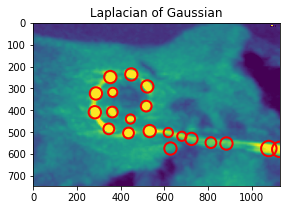
\includegraphics[width=.5\textwidth]{blobs_detected.png}
	\caption{Image after contrast stretching. Red circles indicate locations where blobs have been detected. Radii are approximated using $r=\sqrt{2 \sigma }$.}
	\label{blobs_detected}
\end{figure}
\subsubsection{Blob selection and labelling with MLE}
We used a graph-based approach to distinguish the marked electrodes from other blobs by their distinctive spatial structure and number them in sequence. We made the following assumptions:
\begin{description} %Info
\item[Electrode shape and intensity] The electrodes have a round shape and are brighter than the surrounding tissue. This information was already encoded in the model for blob detection.
\item[Electrode count] There are exactly 12 electrodes to be detected in every image
\item[Equidistance] All the distances between two adjacent electrodes are the same, as they are fixed onto the wire inserted in the cochlea in a regular pattern. Except for the first and last electrode, all electrodes have exactly two neighbours.
\item[Spiral shape] The wire inserted follows the form of the cochlea and is spiral-shaped. The cochlea turns in a regular pattern and has no sharp angles. The electrode density is higher in the center of the cochlea, where the turns get tighter.
\end{description}
\subsubsection{Empirial detection of angle and distance range}
The angles between the electrodes (e.g. between electrode 1,2 and 3) differ among electrodes; therefore, a specific range could be determined empirically: 
\begin{enumerate}
\item The maximal and minimal possible angle between 3 electrodes (ground truth data) was calculated considering the fact that our blob detection could detect blobs deviation by 15pxl from the true blob center. 
\item A confidence interval with confidence level 90 was constructed for every group of three electrodes (assuming a normal distribution), once using the minimal possible angles obtained and once using the maximum angles obtained. These two confidence intervals determined the possible angle range.
\begin{figure}[ht]
	\centering
  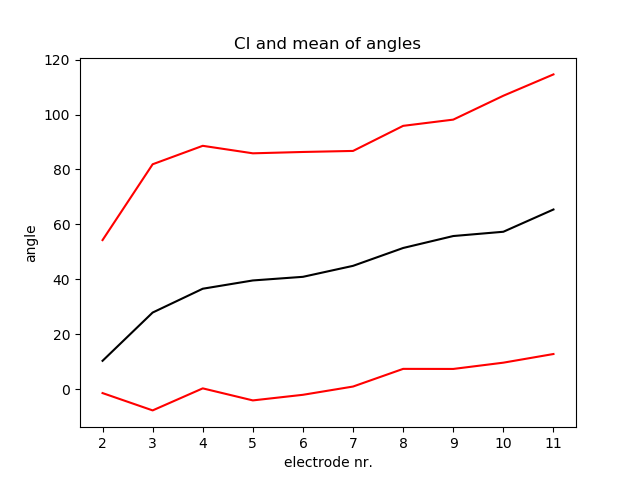
\includegraphics[width=.5\textwidth]{CI_and_mean_of_angles.png}
	\caption{The black line connects the mean angle values, while the red lines connect the CI boundaries at a level of $\alpha$=0.1 of each electrode, considering the possible deviation of our blob detection from the truth.} %TODO
	\label{mean_angles}
\end{figure}
\end{enumerate}
The range in which the distances between the electrodes can be was determined empirically. This was a stronger assumption, as it required the images to show the cochlea in a normalized size. However, as this was approximately given for all received images, it seems reasonable to assume. The confidence interval with confidence level 90 was constructed using all distances (ground truth data, assuming a normal distribution); then the CI was enlarged by two times the possible blob deviation of 15 pixels at both borders (as both electrodes between which the distance was measured could deviate by max 15 pxl (see fig. \ref{dist_distribution}). 
\begin{figure}[ht]
	\centering
  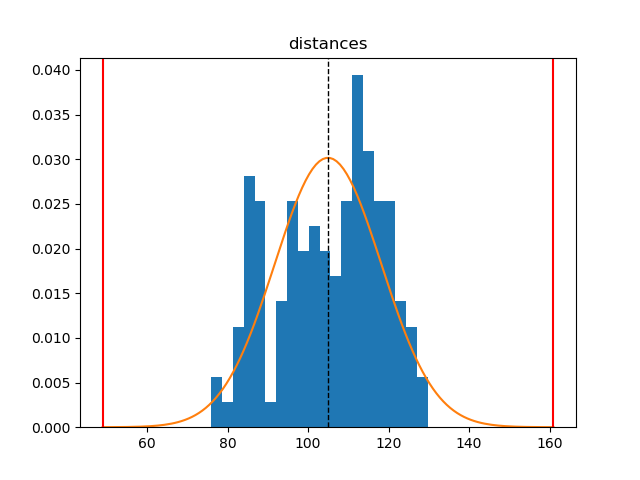
\includegraphics[width=.5\textwidth]{distances_distribution.png}
	\caption{The frequency of all distances, fitted to a normal distribution(orange). The red lines show the border of the CI at a level of $\alpha$=0.1, each extended by 30 due to the possible deviation of our blob detection from the truth} %TODO
	\label{dist_distribution}
\end{figure}
To remove outliers, we calculated the sum of the distances to the other blobs $D_{i}$ for each blob $i$ according to the formula below. Subsequently. We removed the blob that was furthest away from all others. This reduced the number of blobs to $n-1$. We repeated this process until the number of blobs was 20.
%TODO Lucien: Gäu mir hei uf 20 Blobs reduziert? Lucien: "Ja"

$$D_{i}=\sum_{j\neq i}^{n} \sqrt{(b_ix-b_jx)^2+(b_iy-b_jy)^2}$$
A graph representation was created using the \emph{networkX} library \cite{networkx} by assuming each detected blob to be a node. Two blobs were connected with an edge if the distance between them fell into the empirically determined range (see fig. \ref{network_raw}). %TODO Dona
\begin{figure}[ht]
	\centering
  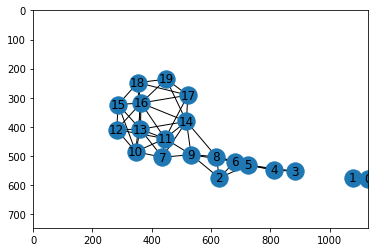
\includegraphics[width=.5\textwidth]{network_raw.png}
	\caption{The initial graph constructed from the blobs in figure \ref{blobs_detected}. The unconnected sub graph containing node 1 will be removed in the following step, see figure \ref{graphs}}
	\label{network_raw}
\end{figure}
Disconnected sub graphs containing less than 12 electrodes were removed. A set of valid paths was generated using the information of the electrode count and spiral shape: Two neighbouring nodes were chosen as starting nodes (this was repeated for all $n$ nodes and all their neighbours). The two starting nodes were used as initialization values of $path_{1...i = len(path)}$ in the recursive function in figure. \ref{pseudo_code}.
%\begin{figure*}
\begin{algorithm*}
	\caption{findpath($graph,path$)} 
	
	\begin{algorithmic}[1]
		\If{$len(path)$ = 12}
			 \State We have found 12 electrodes.
		\Return $path$
		\EndIf
		\State For the node added last to the $path$ check if they have neighbours.
		\For {$node = [all\ neighbours\ of\ path_i, \notin path]$}
				\State Check if we make a plausible turn by choosing this node as continuation of our path:
				\State $\alpha$ = angle between $\overrightarrow{path_{i-1}, path_i}$ and $\overrightarrow{path_i, node}$
				\If{$\alpha$ $<$ empirically determined threshold}
					\State A new possible way to continue this graph has been found, the turn is not to sharp.
					\State $path_{new}$ = Add $node$ to $path$
					\State Recursively call this function with the new path:
					\State \emph{findpath}($graph,path_{new}$)
				\EndIf
		\EndFor
		\If{$node = [\ ]$}
			\State There is no way to continue this path
			\Return
		\EndIf
		
	\end{algorithmic} 
	\label{pseudo_code}
\end{algorithm*}

%\end{figure*}
This lead to a set of paths $P$ where each path $p_i \in P$ was valid to the constraints of having exactly 12 nodes and not making impossible turns. Subsequently, we filtered the paths by assigning a cost function $c_a$ encoding our knowledge about the equidistance of the path: The cost is the variance of the length of all the edges connecting the 12 electrodes in the path $p_i$
$$ c_a(p_i)=var(edges\in p_i)$$
These values were then normalized with min-max normalization for each image. The path with the lowest cost was accepted as the correct solution, giving us the twelve correctly detected electrodes and the order in which they were connected. This already led to really good results in most of the images of the test set. However, in two images there was another path which had a lower edge length variance than the expected solution. The mistake was that these paths started at a wrongfully created point upstream the wire. To penalize these solutions, a second cost function cb was introduced, that measured the ”compactness”. It works by summing up all distances of each node to the mean location of all twelve nodes, assigning less cost to solutions that are nicely curled up, and more cost to solutions that are stretched out.
$$ c_b(p_i)=dist (nodes \in p_i\ to\ center\ of\ mass)$$
The two cost functions were combined into $c_ {c}$. One can think of it as the euclidean distance of the two cost functions from the null point in figure \ref{feature_distribution}.

$$c_{c} = \sqrt{c_a^2+c_b^2}$$

The distribution of $c_a$ and $c_b$ for all valid paths detected in one image are illustrated in figure \ref{feature_distribution}.
\begin{figure}[ht]
	\centering
  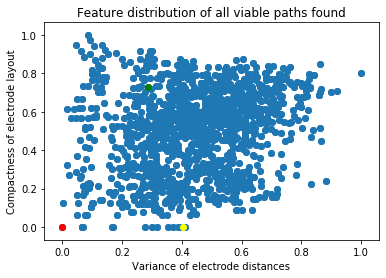
\includegraphics[width=.5\textwidth]{feature_distribution.png}
	\caption{Costs of all paths found in an image. Three paths are highlighted to better illustrate what the dots stand for, and are pictured in the subsequent figures. \textbf{Red:} Best path found (lowest cost for $c_c$), \textbf{Yellow, Green:} Randomly selected.}
	\label{feature_distribution}
\end{figure}

\begin{figure*}[t]
\begin{subfigure}[c]{0.32\textwidth}
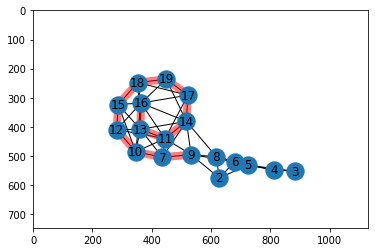
\includegraphics[width=1\textwidth]{best_path.png}
\subcaption{Best path found}
\end{subfigure}
\begin{subfigure}[c]{0.32\textwidth}
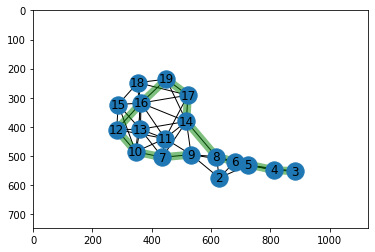
\includegraphics[width=1\textwidth]{random_path_1.png}
\subcaption{Randomly selected path}
\end{subfigure}
\begin{subfigure}[c]{0.32\textwidth}
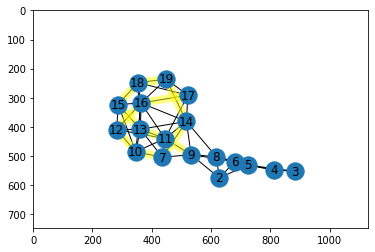
\includegraphics[width=1\textwidth]{random_path_2.png}
\subcaption{Randomly selected path}
\end{subfigure}
\caption{Paths taken from the feature distribution illustrated in figure \ref{feature_distribution}}
\label{graphs}
\end{figure*}
This procedure means each path was detected twice (forwards and backwards). To calculate the angles correctly, it was necessary to start counting at the right node. The starting node was identified by comparing the distance to the electrode center of mass for the first and last node in path.

\subsection{Spectral center}
The spectral center has been approximated as the center of the circle built by the three innermost electrodes\cite{spectral_center}.
$$\overrightarrow{M1}+s*\overrightarrow{n1}=\overrightarrow{M2}+r*\overrightarrow{n2}$$where \overrightarrow{M1} = middle point between electrode 1 and 2, \overrightarrow{M2} = middle point between electrode 2 and 3, s/r= some numbers, \overrightarrow{n1}\ =\ normal vector to the vector connecting electrode 1 and 2, \overrightarrow{n2}\ =\ normal vector to the vector connecting electrode 2 and 3.


\section{Results and discussion}
\subsection{Electrode detection accuracy}
The automatically detected electrode coordinates were compared with the coordinates from the manually annotated ground truth set. The results are illustrated in figure \ref{results_coord}. We were able to detect the electrodes with a high accuracy.
\begin{figure}[ht]
	\centering
  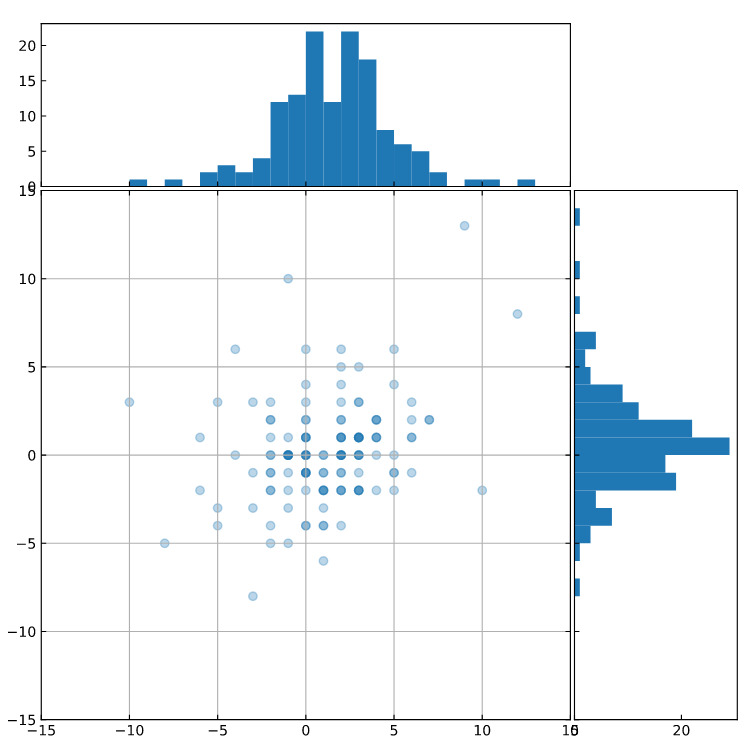
\includegraphics[width=.5\textwidth]{results_coord.jpeg}
	\caption{The x and y pixel deviations of all electrodes in the training dataset from the ground truth dataset.}
	\label{results_coord}
\end{figure}
The result for image \texttt{ID-06} are illustrated in figure \ref{10}, with the corresponding angles given in table \ref{table}. The electrode locations for the full dataset can be found in the appendix \ref{results_complete}.
\begin{figure}[ht]
	\centering
  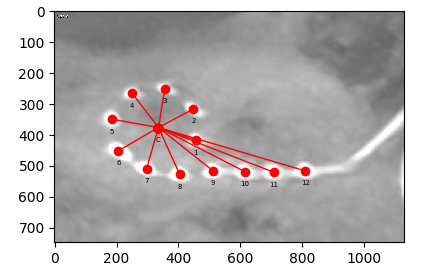
\includegraphics[width=.5\textwidth]{10.png}
	\caption{Detected electrodes and center in image \texttt{ID-06}}
	\label{10}
\end{figure}

\begin{table}[]
\caption{Angular insertion depth of electrodes in image \texttt{ID-06}}
    \label{table}
    \begin{center}
\begin{tabular}{lllll}

\textbf{Electrode} & \textbf{Angle (in degrees)}\\
      \hline
1  & 362.43 &  &  &  \\
2  & 315.57 &  &  &  \\
3  & 262.80 &  &  &  \\
4  & 215.87 &  &  &  \\
5  & 173.60 &  &  &  \\
6  & 133.36 &  &  &  \\
7  & 89.64  &  &  &  \\
8  & 49.16  &  &  &  \\
9  & 22.00  &  &  &  \\
10 & 10.60  &  &  &  \\
11 & 4.75   &  &  &  \\
12 & 0      &  &  & 
\end{tabular}
\end{center}
\end{table}



\subsection{Other approaches explored: CNN}
We have investigated different methods with which the electrodes in the image can be recognized. An exciting discovery was the UNET convolutional neural network, which has recently gained notoriety for its reliable, accurate segmentation of medical images and its ability to achieve excellent results even with limited training data \cite{ronneberger_u-net_2015}. The concept of this architecture is not discussed in detail in this report, as it is not included in the finalized version of our code. We created a training set with postoperative images and corresponding masks of only four examples. This was a very counter-intuitive approach, since more than a hundred times the amount of this data is usually recommended for training neural networks. \cite{hestness_deep_2017,foody_effect_1995}. To counteract overfitting, we used extensive data augmentation and included dropout layers in the architecture \cite{wu_towards_2015}. After training for 300 epochs, we could show very promising results.
\begin{figure}[]
	\centering
  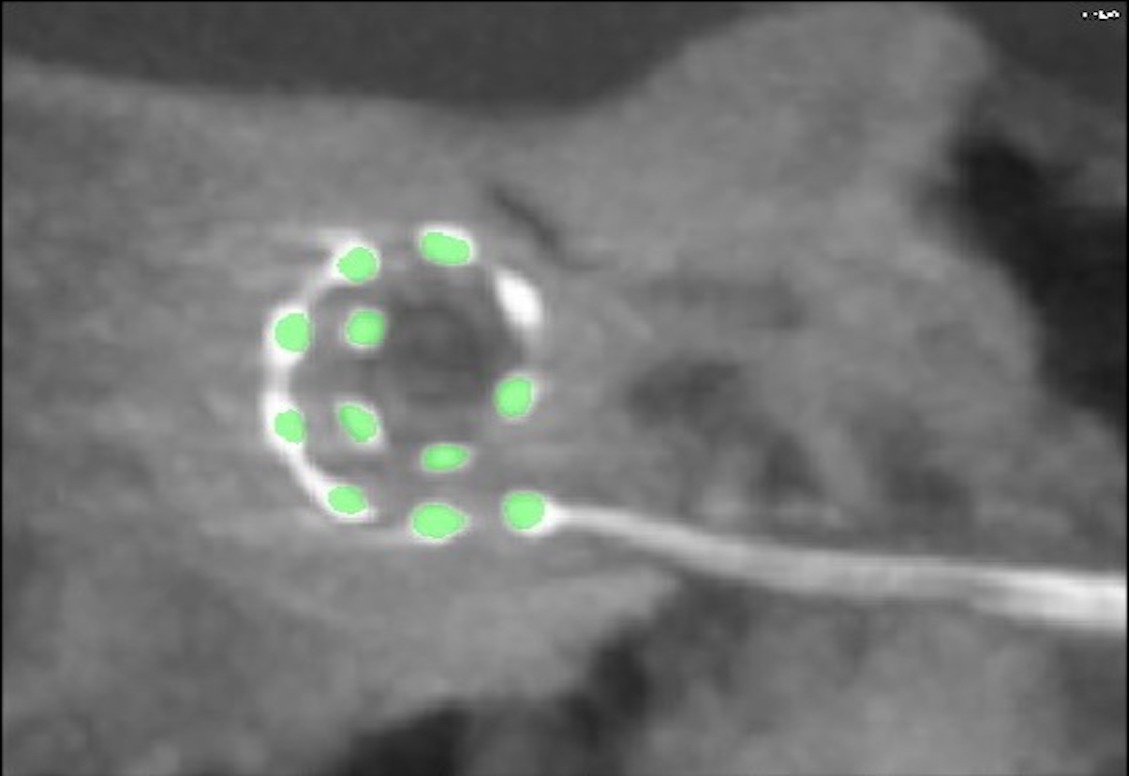
\includegraphics[width=.5\textwidth]{UNET.jpg}
	\caption{Electrode region prediction by UNET. The green mask indicates the region predicted to include the electrodes with a certainty of more than 95\%.}
	\label{UNET}
\end{figure}
In the example in figure \ref{UNET}, eleven of the twelve electrodes were correctly identified in an image that was not used for training the network. This result is quite astonishing considering the small amount of training data. On the one hand, the quality of the result can be attributed to the impressive properties of the UNET, on the other hand it also became clear that this is a rather simple problem. Deep learning approaches have had a difficult time in medicine because of their lack of traceability \cite{litjens_survey_2017}. Thus, we decided to use a less complex algorithm to detect the electrodes, where every step can be followed exactly.
\subsection{Advantages and weaknesses of graph approach}
The use of a graph approach allowed us to be less strict on the blob filtering thresholds. We considered a multitude of other cost functions (e.g. penalizing direction changes, inferring likelihood of angles between specific electrode numbers using empirically determined angle distributions, penalizing crossing edges), but ended up not implementing them, as satisfactory results were already achieved with only two features.
We nevertheless have to point out the very narrow confidence interval (at a level of 90!), which had to be used to prevent certain edges in the graphs from being created. Image ID04 was most critical, because the distance between electrodes 7 and 8 deviated extensively from the other distances and the equidistance assumption was not valid. In this image, a confidence level of 95 for the angles allowed the more evenly spaced edges from electrode 7 to 1 to 8; those were actually preferred by our graph algorithm leading to a wrong result. Of course, when using our algorithm for data where the ground truth is unknown, a CI of 90 could be too restrictive.This problem could be solved using more cost functions as discussed above. 



%TODO add more

\section{Contributions}
The authors have worked very closely together in the realisation of this project. Lucien Hinderling and Tim Ogi investigated different methods for preprocessing and the recognition of the electrodes and finally agreed on the process presented here. Lucien Hinderling developed a graph based approach to realize the numbering of the electrodes. The individual components of the pipeline presented here were configured using data extracted by Tim Ogi from the images available to us and statistically evaluated by Dona Lerena. The calculations of the angles and positions of the electrodes and the centre point were carried out by Dona Lerena.
%feel free to change it

\bibliography{references}
\bibliographystyle{apalike}

\begin{landscape}

\appendix
\section{Results: Electrode and center detection}
\begin{figure}[ht]
    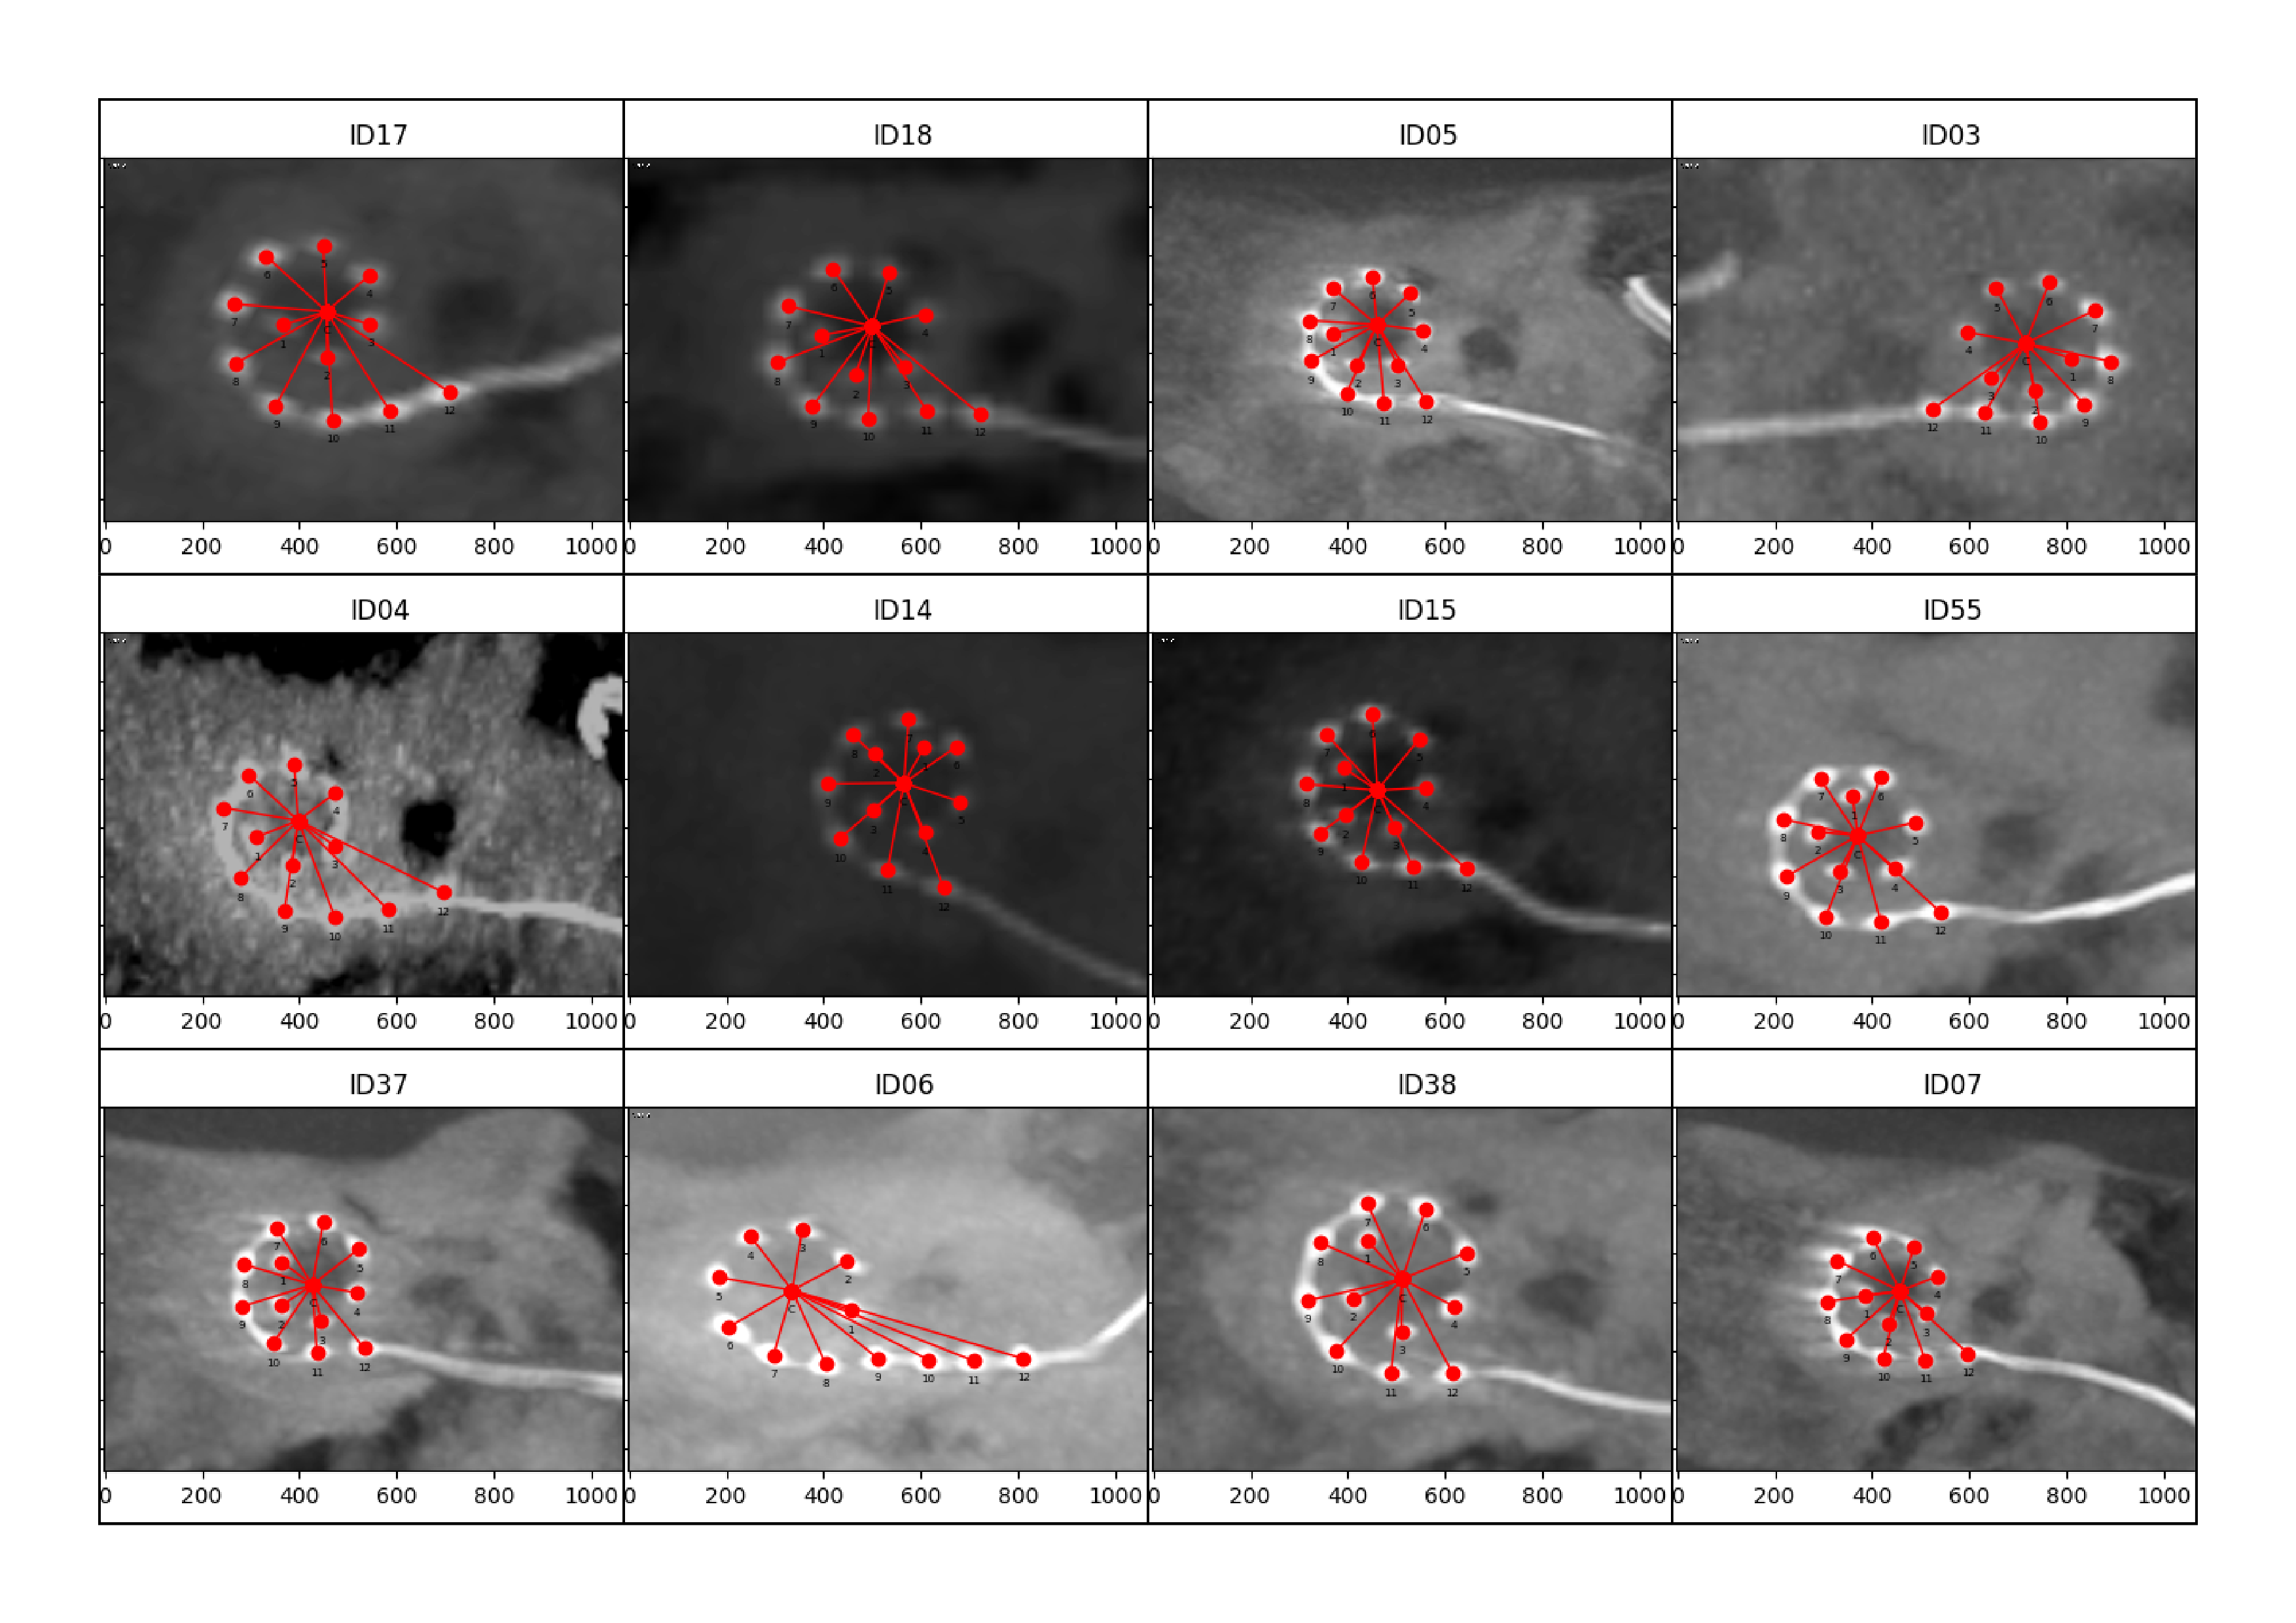
\includegraphics[width=\textwidth]{results.png}
	\caption{Detected electrodes and center for all images in the dataset}
	\label{results_complete}
\end{figure}
\end{landscape}
\end{document}
